\section{Model de dades quasi idèntic a FamilySearch}

    \paragraph{}
    Una altra característica destacable del SDK és que implementa un model de dades equivalent al de l’API de FamilySearch, però en aquest cas, pensat per ser navegat mitjançant els estàndards dels llenguatges de programació orientada a objectes, en comptes dels enllaços hypermedia.

    A la figura~\ref{fig:sdkDataModel} podem observar el model de dades proposat pel SDK i com cada un dels objectes es troba relacionat amb els altres.

    \begin{figure}[h]
        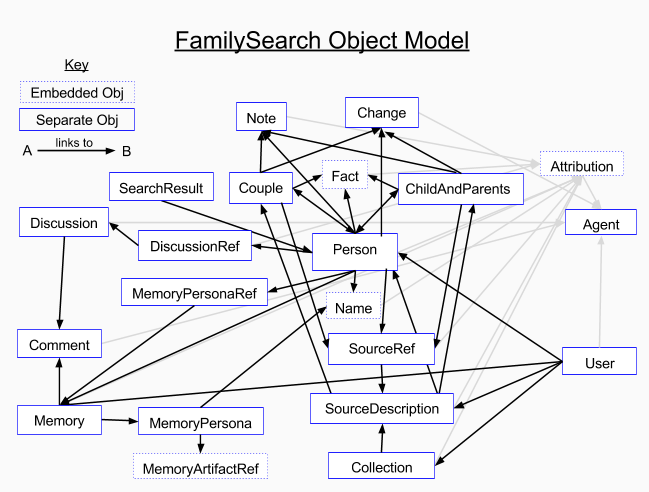
\includegraphics[width=\linewidth]{09/01_objectModel}
        \centering
        \caption{Model de dades del Javascript SDK de FamilySearch}\label{fig:sdkDataModel}
    \end{figure}
